\sloppy
\section{О том, как появилась теория графов...}

\mysubsection{Вначале было слово...}

\epigraph{\itshape Я бы хотел, чтобы мы построили такой мир, 
в котором могли бы контролировать свою информацию, владеть ею.}
{--- Тим Бернерс-Ли, \textit{создатель Всемирной паутины}}

	Единственным критерием выбора, который мы делаем каждую секунду, является наш опыт. Он постоянно меняется под
	влиянием информации, которую мы впитываем из окружающего нас мира. Именно поэтому, <<кто владеет информацией, тот владеет миром>>
	(Натан Ротшильд, \emph{основатель банковской династии Ротшильдов}).
	
	Мы же живем сейчас в мире цифровых технологий, где нас окружило невероятное множество телефонов, компьютеров и прочих электронных устройств.
	Из-за этого мы должны очень тщательно подходить к выбору той информации, которой нас кормят СМИ, блогеры, газеты... В частности 
	с недавнего времени Интернет вышел на первое место в списке источников информации. Этот очень сложный механизм, которым мы ежедневно
	пользуемся, дает нам столько возможностей, что мы иногда забываем о других не менее приятных процессах. Поэтому чтобы не оказаться в
	информационной ловушке, полезно знать хотя бы поверхностно его устройство. 
	
	Я не собираюсь здесь читать нравоучения о том, что правда, а что ложь, из того объема, который приходит к нам из Всемирной паутины.
	Моя цель~---~познакомить читателя с частью объектов и механизмов, которые были заложены в процессе разработки ПО, поисковых машин,
	блокчейнов... Главный герой моего рассказа~---~граф, математический объект. Нельзя раскрыть его сущность, не рассказав при этом о
	его рождении и периоде становления теории, в которую он обличен.
	
	Именно этому и посвящены следующие несколько страниц.

\mysubsection{История развития}

	Исследователи математики сходятся во мнении, что мать теории графов~---~комбинаторика~---~возникла в \RNumb{16} веке.
	Конечно, есть некоторые предпосылки считать, что еще в Древнем Китае использовали комбинаторный анализ для изучения игр, 
	однако из-за упадка в Средние Века культуры, письменности и науки ученым, в том числе и математикам, впоследствии пришлось 
	открывать всё с нуля. Тоже самое можно сказать и о теории алгоритмов: несмотря на то что до нас дошел алгоритм Евклида, 
	появление которого датируется \RNumb{3} веком до н. э., но эта теория начала развиваться только в \RNumb{20} веке.
	
	Первые комбинаторные задачи касались азартных игр, отвечая на вопросы: каков шанс, что выпадет данное число очков; 
	какая стратегия является выигрышной? Именно повсеместное увлечение азартными играми высших слоев общества стало движущей силой в
	развитии комбинаторной дисциплины. Такое положение дел неплохо описано в <<Комбинаторике>> Н. Я. Виленкина, П. А. Виленкина, А. Н. Виленкина:
	
\begin{displayquote}
	\textit{Большим подспорьем для математиков являлось то, что решение задач такого рода можно было проверять на практике~---~во время игр. 
	Зачастую происходило так, что во время многочасовых игр замечались определенные закономерности (например, что определенные комбинации карт 
	или костей появляются чаще других), о которых игроки сообщали математикам, а последние объясняли эти наблюдения.}
\end{displayquote}

	Попутно возникало невероятное количество задач на подсчёт, которые требовали для своего решения появления нового математического аппарата. 
	Так, в $1527$ году в печать вышла книга Петра Апиана <<Новом и хорошо обоснованном наставлении по арифметике для всех купцов>> 
	(Eyn Newe Vnnd wolgegründte vnderweysung aller Kauffmanß Rechnung), в которой впервые были упомянуты биномиальные коэффициенты. Дальше укрепляли
	позиции комбинаторики такие известные ученые, как Никколо Тарталья, Джероламо Кардано, Блез Паскаль, Пьер Ферма и другие.
	
	За свою $500$-летнюю историю комбинаторика расширяла свои владения, завладев частью теории экстремальных задач, топологии, теории вероятностей, 
	теории игр, экономики, социологии. Кроме такой экспансии, она породила ещё несколько своих направлений: 
	теорию графов, теорию Рамсея, перечислительную комбинаторику.
	
	Достоверно известно, что впервые теория графов была затронута в одной из работ Леонарда Эйлера, опубликованной в $1736$ году. 
	В ней Эйлер сформулировал и решил <<Задачу о семи кёнигсбергских мостах>>. Как и всегда, математические головоломки использовались 
	скорее в качестве развлечения и не предвещали новые открытия, поэтому долгое время теория графов не имела широкого применения 
	и не воспринималась всерьёз.  

	Однако некоторые всё-таки преуспели в этом деле. Так, например, в $1852$ году Фрэнсисом Гутри была сформулирована гипотеза о четырёх красках.
	Понадобилось почти $120$ лет, чтобы решить её. Позже мы ещё вернемся к обсуждению ее.
	
	В XIX веке произошёл значительный скачок в теории графов, связанный с развитием теории электрических цепей и органической химии. 
	В~$1847$ году Густав Кирхгов доказал матричную теорему о деревьях, а в~$1889$ году Артур Кэли, английский математик, доказал одноименную
	теорему о числе остовных деревьев полного графа. С начала $30$-х годов \RNumb{19} века математики, как голодные звери, постепенно стягивались 
	на эту сладкую и новую область, в которой, как оказалось, далеко не всё было очевидным.
	
	В свою очередь, появление теории алгоритмов ассоциируют с работой Курта Геделя, опубликованной в $1931$ году, в которой была доказана теорема 
	о неполноте исчисления предикатов. Вслед за этим последовал ряд фундаментальных работ, написанных Аланом Тьюрингом, Алоизом Черчем и Эмилем Постом.
		
	В середине \RNumb{20} века и теория графов, и теория алгоритмов вошли в авангард математики. Этот период связан с такими 
	известными исследователями теории алгоритмов, как Колмогоров, Марков, Кнут, и с не менее известными учеными, которые развивали
	теорию графов: Оре, Холл, Берж, Харари. В последние $30$ лет эти два направления приобрели невероятные масштабы в связи с 
	появлением Всемирной паутины, созданной Тимом Бернерс-Ли в $1989$ году.

\begin{center}\begin{tikzpicture}
	\draw[->] (-8,0) -- (8,0) node [below] {}; % Временная ось
    \foreach \x/\d/\t in {-7.5/1527/Апиан П., -5.5/1736/Эйлер Л., -3/\RNumb{19} век/\text{Кирхгов, Кэли}, 
    1.5/сер. \RNumb{20} века/\text{Харари, Колмогоров}, 6.5/1989/Тим Бернерс-Ли}
        \draw (\x, 0.1) -- (\x, -0.1) node [below] {\shortstack{\d\\ \t}}; % Даты и имена
\end{tikzpicture}

	\small Рис. \images. Временная шкала с основными датами развития теории графов и теории алгоритмов
\end{center}

	Благодаря элегантному, стройному виду, в который облачили теорию графов и теорию алгоритмов математики середины и конца \RNumb{20} века,
	их начали активно использовать при составлении олимпиад для школьников и студентов, включили во многие студенческие программы. Такая 
	практика только укрепила фундамент этих теорий и дала толчок к появлению большого числа методических пособий, направленных на 
	неподготовленного читателя. До сих пор скорость развития теории графов и теории алгоритмов не снизилась.
	
	С этого момента мы забудем об алгоритмах на время и вернемся к ним уже в третьей главе. 
	Хотя во время изучения элементов теории графов, мы столкнемся с некоторыми несложными алгоритмами.
	

	На этом моменте я хочу сделать небольшое лирическое отступление и задать риторический вопрос: как происходит развитие математической науки?
	
	Сначала есть некоторые простые головоломки, загадки, которые не поддаются быстрому <<взлому>>. И чтобы их решить, 
	начинают создавать новый математический инструмент. Так, появляется база (на рис. ниже это маленький кружочек слева). 
	Далее ее начинают развивать и приходят к утверждениям, которые не могут доказать (точки на рис. ниже, в центральной части). 
	Возникают области вокруг этих математических задач (на рис. ниже это области в центральной части), которые, может быть, успешно 
	доказывают поставленную задачу. Вскоре математики замечают взаимосвязь между областями, начинают структуризовать науку, 
	приходят к единым понятиям, обозначениям и объединяют эти разрозненные области (на рис. ниже это большая закрашенная область справа).

\begin{center}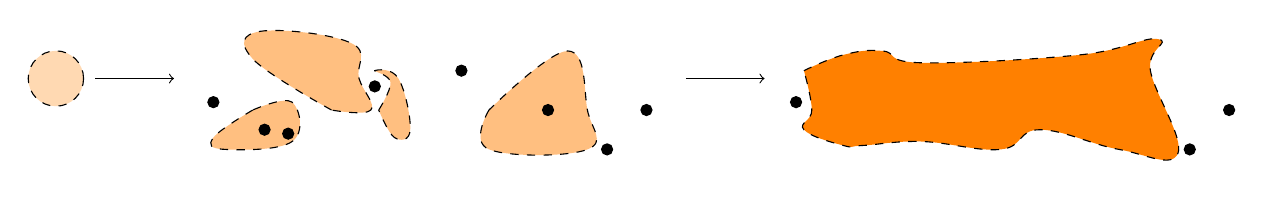
\begin{tikzpicture}[scale=0.50]
	\node [dashed] at (-14,0.8)[shape=circle, draw, fill=orange!30,inner sep=4pt] {}; % Левый круг

	\draw [->] (-13, 0.8) -- (-11, 0.8); % Левая стрелка

	% Оранжевые области по центру
	\draw [dashed,fill=orange!50]  plot[smooth, tension=.7] coordinates {(-3,0) (-3,-1) (-0.5,-1) (-0.5,0) (-1,1.5) (-3,0)};
	\draw [dashed,fill=orange!50]  plot[smooth, tension=.7] coordinates {(-7,0) (-9, 1.3) (-8.8,2) (-6.5,1.7) (-6.3,0.8) (-6,0) (-7,0)};
	\draw [dashed,fill=orange!50]  plot[smooth, tension=.7] coordinates {(-5.8,0) (-5.5,0.7) (-5.9,1) (-5.3,0.8) (-5,-0.5) (-5.4,-0.7) (-5.8,0)};
	\draw [dashed,fill=orange!50]  plot[smooth, tension=.7] coordinates {(-9,0) (-10,-0.7) (-9.7,-1) (-8,-0.8) (-8,0.2) (-9,0)};
	
	% Точки по центру
	\tikzstyle{every node}=[circle, draw, fill=black, inner sep=0pt, minimum width=4pt]	
	
	\node at (-5.9,0.6) {};
	\node at (-8.1,-0.6) {};
	\node at (-8.7,-0.5) {};
	\node at (-1.5,0) {};
	\node at (0,-1) {};
	\node at (1,0) {};
	\node at (-10,0.2) {};
	\node at (-3.7,1) {};

	\draw [->] (2, 0.8) -- (4, 0.8); % Правая стрелка

	% Большая область справа
	\draw [dashed,fill=orange]  plot[smooth, tension=.7] coordinates {(5, 1) (6, 1.4) (7, 1.5) (8, 1.2) (12, 1.4) 
	(14, 1.8) (13.8, 1) (14.5, -1.1) (13, -1) (11, -0.5) (10, -1) (8, -0.8) (6.5, -0.9) (6, -0.9) (5, -0.5) (5.2, 0) (5, 1)};	
	
	% Точки справа
	\node at (14.8,-1) {};
	\node at (15.8,0) {};
	\node at (4.8,0.2) {};
\end{tikzpicture}

	\small Рис. \images. Схематическое изображение развития какой-нибудь области математики
\end{center}

	Как мог уже заметить читатель, по таком пути развития прошла и теория графов. В ее случае начало было заложено Эйлером в 1736 году. 
	К середине \RNumb{19} века в этой теории было найдено много нетривиальных теорем, часть из которых не могли доказать. 
	К концу \RNumb{20} века и по нынешнее время продолжается процесс структуризации всех ранее разрозненных областей теории графов.

	И это не единичный случай. Имеется достаточно областей, в которых в течение нескольких веков разрасталась теория с 
	единственной целью~---~решить великую математическую задачу. Стоит только вспомнить нашумевшую в конце \RNumb{20} века 
	Великую теорему Ферма, которую всё-таки смог в $1994$ году доказать Эндрю Уайлс. Однако между доказанной и недоказанной 
	теоремой мало отличий, с практической точки зрения, а значит, и пользы мало от завершения доказательства. Так что главный 
	результат стараний математиков~---~это создание вокруг поставленных задач, иногда гигантских, теорий, которые впоследствии 
	или в процессе находят себе многочисленное прикладное значение.
	
\begin{paracol}{2}
	Как мы только что осознали, в становлении теории графов большую роль сыграла практика. Как именно? Когда специалист сталкивался с 
	какими-то операциями, связями, отношениями, он пытался их изобразить в качестве рисунка. При этом суть самих вещей опускалась, 
	то есть было не важно, как изобразить объект, поэтому было удобно для этого на рисунке поставить просто точку.
	
	Далее надо было указать отношения между этими точками и вполне логично было соединять точки линиями. 
	В некоторых ситуациях, чтобы указать отличительную особенность отношений между объектами, стоило рисовать вместо линии стрелку.
	
	Таким образом, и начали появлятся графы~---~рисунки с вершинами, некоторые из которых соединены линиями.
	 
\switchcolumn

\begin{tikzpicture}
	% Два изогнутых ребра
	\path (144:1.5) edge [bend right=45](216:1.5)
    	  (144:1.5) edge [bend left=30] (288:1.5);	
   	 
   	% Петли в вершинах пятиугольника
	\Loop [dist=2cm, dir=EA](0:1.5);
	\Loop [dist=2cm, dir=NO](72:1.5);
	\Loop [dist=2cm, dir=NOWE](144:1.5);
	\Loop [dist=2cm, dir=SOWE](216:1.5);
	\Loop [dist=2cm, dir=SOEA](288:1.5);
	
	% Нижняя петля
	\Loop [dist=2cm, dir=NO](260:5);  
	
	% Пятиугольник	
	\tikzstyle{every node}=[circle, draw, fill=red, inner sep=0pt, minimum width=6pt]	
	\foreach \x in {0,72,...,288}
    {
    	\draw [->, >=stealth']
    	(\x:1.5) node {} -- (\x+72:1.5)
    	(\x:1.5) node {} -- (\x+144:1.5)
    	(\x:1.5) node {} -- (\x+216:1.5)
    	(\x:1.5) node {} -- (\x+288:1.5);
    };
    
    % Нижняя часть графа
    \draw (255:2.5) node {} -- (285:4.5) node {} -- (265:6) node {} -- (260:5) node {};
      
    % Перерисовываем вершины, чтобы концы стрелок не залезали на них
    \draw \foreach \x in {0,72,...,288}
    {
    	(\x:1.5) node {}
    };
\end{tikzpicture}\begin{center}
	\small Рис. \images. Абсолютно произвольный граф 
\end{center} \end{paracol}
\refstepcounter{images} 
	
	После того, как задача формулировалась на языке теории графов, математики указывали параметры, которые были весомыми 
	в рамках поставленной задачи. Так, в каких-то задачах надо было изображать ориентированные графы, в других~---~планарные, 
	в тех, которые были связаны с сетями,~---~взвешенные, случайные. С помощью расширения области применения графов вариативность 
	графов расширялась, открывая невероятные миры перед математиком.	 

	Математики отвечали взаимностью на такое разнообразие графов: у них появлялось невероятное число вопросов, на которые должна 
	была ответить теория графов. Смешение возможностей этой новой области и рвения самых любопытных математиков привело к тому, 
	что графы заняли одно из самых главных мест в комбинаторике. 

	Всё, пришло время окунуться в мир теоретико-графовых моделей!

\mysubsection{Примеры}	

	Разберём три примера, которые можно отнести к самому нижнему ярусу школьной олимпиадной математики. 
	Они покажут нам, как с помощью несложных рассуждений в рамках теории графов можно буквально разломить задачу и достать искомый ответ.
	
	Два примера позаимствованы из книги <<Ленинградские математические кружки>>, а один из книги <<Как решают нестандартные задачи>>, 
	в которых любознательный читатель может найти много схожих интересных задач. В этих книгах также увлекательно изложены многие темы, 
	которые было бы полезно освоить начинающему олимпиаднику.
	
\begin{example}
	Между $9$-ю городами России введены участки высокоскоростной автомагистрали. Есть следующие марщруты: 
	Москва~---~Казань, Владивосток~---~Архангельск, Москва~---~Владивосток, Владивосток~---~Казань, Казань~---~Архангельск, 
	Грозный~---~Смоленск, Смоленск~---~Новгород, Новгород~---~Углич, Углич~---~Тверь и Тверь~---~Грозный. 
	Можно ли добраться из Москвы до Твери?

	\emph{Решение.} Нарисуем схему: городами будут соответственно точки, а соединяющим их дорогами~---~непересекающиеся
	между собой линии (см. рис. $4$). Теперь видно, что доехать от Москвы до Твери нельзя.

\begin{center}\begin{tikzpicture}
		[shorten >=1pt,auto,node distance=1.7cm, thick, main node/.style={circle,draw, font=\sffamily, minimum width=16pt}]
  		
  		% Правый граф
		\node[main node] (Z) 		   	   {М};
  		\node[main node] (P)  [below of=Z] {В};
  		\node[main node] (Me) [right of=Z] {К};
  		\node[main node] (V)  [right of=P] {А};
  		
 		\draw
    	(Z)  -- (Me)
    	(Me) -- (P)
    	(P)  -- (Z)
    	(P)  -- (V)
    	(V)  -- (Me);
    	
    	\draw (6, -3.2) node {};
\end{tikzpicture}
\begin{tikzpicture}
		[shorten >=1pt,auto,node distance=1.7cm, thick, main node/.style={circle,draw, font=\sffamily, minimum width=16pt}]
  		
  		% Левый граф
  		\node[main node] (U)  [] {Г};
  		\node[main node] (N)  [above of=U] {С};
  		\node[main node] (S)  [right of=N] {Н};
  		\node[main node] (Ma) [right of=U] {Т};
  		\node[main node] (J)  [below right of=S] {У};
  		
 		\draw
    	(U)  -- (N)
    	(N)  -- (S)
    	(S)  -- (J)
    	(J)  -- (Ma)
    	(Ma) -- (U);
    	
    	\draw (0, -1.5) node {};
\end{tikzpicture}\end{center}
\begin{center}
	\small Рис. \images. Высокоскоростные магистрали
\end{center}
\end{example}

\begin{example}
	Можно ли за несколько ходов из исходного положения (см. рис. $5$) получить такую же картину, как на рис. $6$? 

\begin{paracol}{2}
	Занумеруем поля шахматной доски так, как показано на рис. $7$. И представим её в виде графа, в котором будет $9$ вершин
	и соединены будут те из них, которые могут быть последовательными клетками пути коня, то есть отстающие друг от друга на 
	две клетки по вертикали и одну по горизонтали или наоборот. 
	
	Начальная и конечная расстановки изображены соответственно на рис. $8$ и на рис.~$9$. 
	Очевидно, что порядок следования коней измениться не может, поэтому переставить коней не получится.

\switchcolumn

\begin{center}
\begin{tikzpicture}
	% Левый рисунок
	\draw[dashed] (0,0)rectangle (0.5,-0.5);
	\draw[dashed] (0.5,0)rectangle (1,-0.5);
	\draw[dashed] (1,0)rectangle (1.5,-0.5);

	\draw[dashed] (0,-0.5)rectangle (0.5,-1);
	\draw[dashed] (0.5,-0.5)rectangle (1,-1);
	\draw[dashed] (1,-0.5)rectangle (1.5,-1);
	
	\draw[dashed] (0,-1)rectangle (0.5,-1.5);
	\draw[dashed] (0.5,-1)rectangle (1,-1.5);
	\draw[dashed] (1,-1)rectangle (1.5,-1.5);

	\node at (0.25, -0.25)[] {
\includegraphics[width=1in,%
height=0.4cm,keepaspectratio]{chapters/1/images/white_hourse}};
	\node at (1.25, -0.25)[] {
\includegraphics[width=1in,%
height=0.4cm,keepaspectratio]{chapters/1/images/white_hourse}};
	\node at (1.25, -1.25)[] {
\includegraphics[width=1in,%
height=0.4cm,keepaspectratio]{chapters/1/images/black_hourse}};
	\node at (0.25, -1.25)[] {
\includegraphics[width=1in,%
height=0.4cm,keepaspectratio]{chapters/1/images/black_hourse}};	
\end{tikzpicture}
\;\ \;\ \;\
\begin{tikzpicture}  
	% Правый рисунок  
	\draw[dashed] (0,0)rectangle (0.5,-0.5);
	\draw[dashed] (0.5,0)rectangle (1,-0.5);
	\draw[dashed] (1,0)rectangle (1.5,-0.5);

	\draw[dashed] (0,-0.5)rectangle (0.5,-1);
	\draw[dashed] (0.5,-0.5)rectangle (1,-1);
	\draw[dashed] (1,-0.5)rectangle (1.5,-1);
	
	\draw[dashed] (0,-1)rectangle (0.5,-1.5);
	\draw[dashed] (0.5,-1)rectangle (1,-1.5);
	\draw[dashed] (1,-1)rectangle (1.5,-1.5);

	\node at (0.25, -0.25)[] {
\includegraphics[width=1in,%
height=0.4cm,keepaspectratio]{chapters/1/images/white_hourse}};
	\node at (1.25, -0.25)[] {
\includegraphics[width=1in,%
height=0.4cm,keepaspectratio]{chapters/1/images/black_hourse}};
	\node at (1.25, -1.25)[] {
\includegraphics[width=1in,%
height=0.4cm,keepaspectratio]{chapters/1/images/white_hourse}};
	\node at (0.25, -1.25)[] {
\includegraphics[width=1in,%
height=0.4cm,keepaspectratio]{chapters/1/images/black_hourse}};
\end{tikzpicture}

 \;\ \;\ \;\ \;\ \;\ \small Рис. \images \;\ \;\ \;\ \;\ \;\ \;\ \small Рис. \images
\newline
\newline
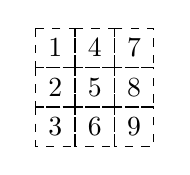
\begin{tikzpicture}    
	% Нижний рисунок
	\draw[dashed] (0,0)rectangle (0.5,-0.5);
	\draw[dashed] (0.5,0)rectangle (1,-0.5);
	\draw[dashed] (1,0)rectangle (1.5,-0.5);

	\draw[dashed] (0,-0.5)rectangle (0.5,-1);
	\draw[dashed] (0.5,-0.5)rectangle (1,-1);
	\draw[dashed] (1,-0.5)rectangle (1.5,-1);
	
	\draw[dashed] (0,-1)rectangle (0.5,-1.5);
	\draw[dashed] (0.5,-1)rectangle (1,-1.5);
	\draw[dashed] (1,-1)rectangle (1.5,-1.5);

	\node at (0.25, -0.25)[] {1};
	\node at (0.25, -0.75)[] {2};
	\node at (0.25, -1.25)[] {3};
	
	\node at (0.75, -0.25)[] {4};
	\node at (0.75, -0.75)[] {5};
	\node at (0.75, -1.25)[] {6};
	
	\node at (1.25, -0.25)[] {7};
	\node at (1.25, -0.75)[] {8};
	\node at (1.25, -1.25)[] {9};
	
\end{tikzpicture}

	\small Рис. \images
\end{center}
\end{paracol}
\begin{center}\begin{tikzpicture}
		[shorten >=1pt,auto,node distance=1.3cm, thick, main node/.style={circle,draw, font=\sffamily, minimum width=20pt}]
  		
  		\node[main node] (a)  [] {
\includegraphics[width=1in,%
height=0.4cm,keepaspectratio]{chapters/1/images/white_hourse}};
  		\node[main node] (b)  [above of=a] {6};
  		\node[main node] (c)  [above right of=b] {
\includegraphics[width=1in,%
height=0.4cm,keepaspectratio]{chapters/1/images/white_hourse}};
  		\node[main node] (d) [right of=c] {2};
  		\node[main node] (e)  [right of=d] {
\includegraphics[width=1in,%
height=0.4cm,keepaspectratio]{chapters/1/images/black_hourse}};
  		\node[main node] (f)  [below of=e] {4};
  		\node[main node] (g)  [below left of=f] {
\includegraphics[width=1in,%
height=0.4cm,keepaspectratio]{chapters/1/images/black_hourse}};
  		\node[main node] (h)  [left of=g] {8};
  		
  		\node[main node] (i)  [right of=g] {5};
  		
 		\draw (a)  -- (b) -- (c) -- (d) -- (e) -- (f) -- (g) -- (h) -- (a);
\end{tikzpicture}
\;\ \;\ \;\ \;\ \;\ \;\ \;\ \;\ \;\ \;\
\begin{tikzpicture}
		[shorten >=1pt,auto,node distance=1.3cm, thick, main node/.style={circle,draw, font=\sffamily, minimum width=20pt}]
  		
  		\node[main node] (a)  [] {
\includegraphics[width=1in,%
height=0.4cm,keepaspectratio]{chapters/1/images/white_hourse}};
  		\node[main node] (b)  [above of=a] {6};
  		\node[main node] (c)  [above right of=b] {
\includegraphics[width=1in,%
height=0.4cm,keepaspectratio]{chapters/1/images/black_hourse}};
  		\node[main node] (d) [right of=c] {2};
  		\node[main node] (e)  [right of=d] {
\includegraphics[width=1in,%
height=0.4cm,keepaspectratio]{chapters/1/images/white_hourse}};
  		\node[main node] (f)  [below of=e] {4};
  		\node[main node] (g)  [below left of=f] {
\includegraphics[width=1in,%
height=0.4cm,keepaspectratio]{chapters/1/images/black_hourse}};
  		\node[main node] (h)  [left of=g] {8};
  		
  		\node[main node] (i)  [right of=g] {5};
  		
 		\draw (a)  -- (b) -- (c) -- (d) -- (e) -- (f) -- (g) -- (h) -- (a);
\end{tikzpicture}\newline \refstepcounter{images}\refstepcounter{images}\refstepcounter{images}
\small Рис. \images  \;\ \;\ \;\ \;\ \;\ \;\ \;\ \;\ \;\ \;\ \;\ \;\ \;\ \;\ \;\ \;\ \;\ \;\ \;\ \;\ \;\ \;\ \;\ \;\ \;\ \small Рис. \images \;\ \;\ \;\ \;\ \;\ \;\ 
\end{center}
\end{example}

\begin{example}
	Можно ли выписать в ряд цифры от 1 до 9 так, чтобы число, составленное из двух соседних цифр, делилось на одно из чисел: 7 или 13?
	
	\emph{Решение.} Можно, это будет число $784913526$. Как его получить? На этот вопрос мы сейчас ответим.

\begin{paracol}{2}	
	Для этого напишем числа на листе и соединим стрелками те пары цифр, которые подходят под условие. Притом стрелка будет идти от цифры, стоящей в старшем разряде, к цифре, стоящей в младшем разряде.
	
	Теперь с помощью нехитрых логических рассуждений можно найти путь, который обходит все вершины, начинаясь с семерки (на рис. справа этот путь обозначен красными стрелками).

\switchcolumn

\begin{center}\begin{tikzpicture}
		[shorten >=1pt,auto,node distance=1.3cm, thick, main node/.style={circle,draw, font=\sffamily, minimum width=16pt}]
  		
  		\node[main node] (a)  [] {7};
  		\node[main node] (b)  [right of=a] {8};
  		\node[main node] (c)  [above of=b] {9};
  		\node[main node] (d)  [right of=c] {1};
  		\node[main node] (e)  [above of=d] {3};
  		\node[main node] (f)  [below of=d] {4};
  		\node[main node] (g)  [below of=f] {2};
  		\node[main node] (h)  [right of=f] {5};
  		\node[main node] (i)  [right of=h] {6};
  		
 		\draw [-latex] (i) -- (h);
 		\draw [-latex] (h) -- (i);
 		\draw [-latex] (i) -- (e);
 		\draw [-latex] (e) -- (c);
 		\draw [-latex] (c) -- (b); 
 		\draw [-latex] (d) -- (f); 
 		\draw [-latex] (f) -- (g);
 		\draw (g) edge [-latex, bend right=45] (d); 

 		\draw (a) edge [-{Latex[color = red,length=1mm,width=2mm]}, line width=0.3mm, color = red] (b)
 			  (b) edge [-{Latex[color = red,length=1mm,width=2mm]}, line width=0.3mm, color = red] (f)
 			  (f) edge [-{Latex[color = red,length=1mm,width=2mm]}, line width=0.3mm, color = red] (c)
 			  (c) edge [-{Latex[color = red,length=1mm,width=2mm]}, line width=0.3mm, color = red] (d)
 			  (d) edge [-{Latex[color = red,length=1mm,width=2mm]}, line width=0.3mm, color = red] (e)
 			  (e) edge [-{Latex[color = red,length=1mm,width=2mm]}, line width=0.3mm, color = red] (h)
 			  (h) edge [-{Latex[color = red,length=1mm,width=2mm]}, line width=0.3mm, color = red] (g)
 			  (g) edge [-{Latex[color = red,length=1mm,width=2mm]}, line width=0.3mm, color = red] (i);
\end{tikzpicture}

	\small Рис. \images
\end{center}\end{paracol}\end{example}\refstepcounter{images}

\mysubsection{Великие математические задачи}

	\textbf{Проблема семи мостов Кёнигсберга} была решена Эйлером в $1736$ году. Это считается отправной точкой появления теории графов. 
	В этой задаче спрашивалось, можно ли пройти по всем семи мостам Кёнигсберга, не проходя ни по какому из них дважды. 
	Многие жители любили эту загадку, но никто не мог ни решить её, ни опровергнуть. 
	
	Эйлер, в свою очередь, переформулировал эту задачу в терминах теории графов: можно ли выйти из какой-то вершины графа и 
	пройти по всем ребрам графа ровно по одному разу. Граф, в котором так можно сделать, называется эйлеровым. 

	На самом деле, как, может, знает любознательный читатель, эйлеров граф~---~это граф, который можно нарисовать на бумаге, не отрывая карандаша. 
	Таким образом, все рисунки из детских раскрасок, у которых надо было нарисовать контур, не отрывая карандаша от бумаги, есть ни что иное, 
	как изображение эйлерового графа. 

\begin{center}
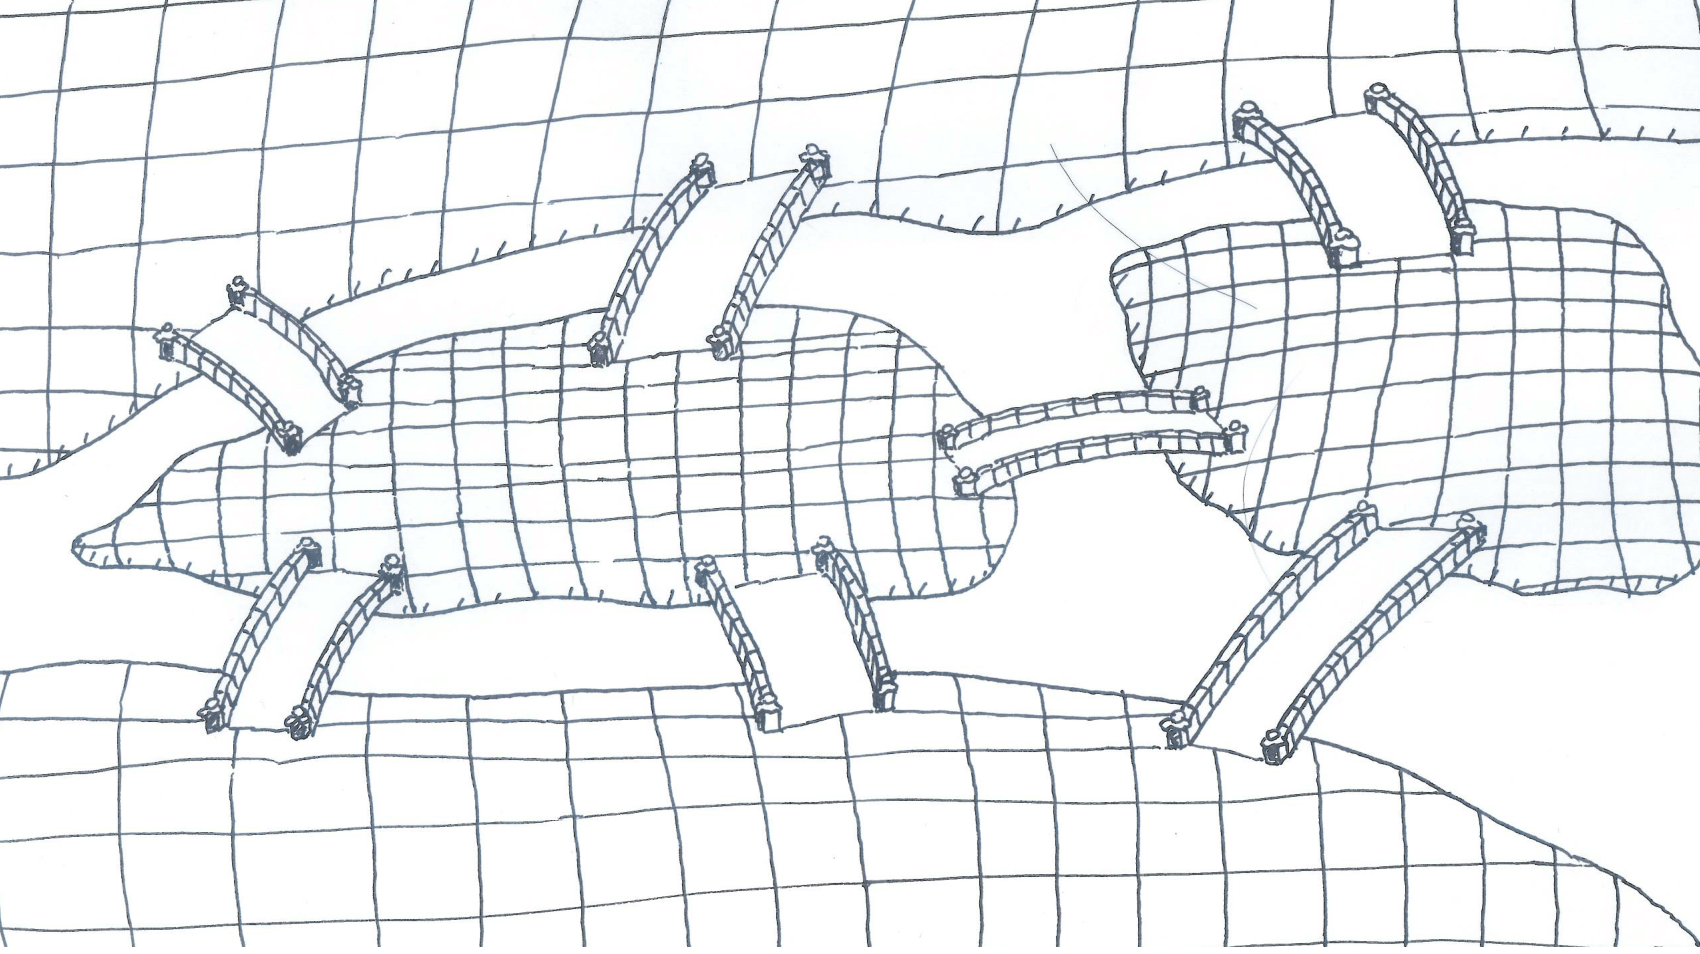
\includegraphics[width=8cm, height=9cm,keepaspectratio]{chapters/1/images/Keningsberg}
\;\ \;\ \;\ \;\ \;\ \;\ \;\ \;\ \;\ \;\
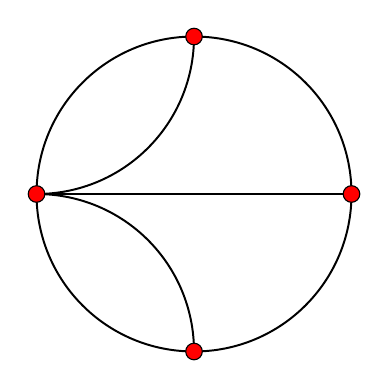
\begin{tikzpicture}
	\tikzstyle{every node}=[circle, draw, fill=red, inner sep=0pt, minimum width=6pt]
    	  
   	\path (0, 0) edge [bend right=45, line width=0.25mm](2, 2)
    	  (0, 0) edge [bend left=45, line width=0.25mm] (2, 2)
    	  (0, 0) edge [bend right=45, line width=0.25mm](2, -2)
    	  (0, 0) edge [bend left=45, line width=0.25mm] (2, -2);	
    	  
	\draw (0, 0) edge [line width=0.25mm] (4, 0)
		  (2, 2) edge [bend left=45, line width=0.25mm] (4, 0)
		  (2, -2) edge [bend right=45, line width=0.25mm] (4, 0);
	
    \draw (0, 0) node {} 
    	  (2, -2) node {} 
    	  (2, 2) node {} 
    	  (4, 0) node {};

\end{tikzpicture}\end{center}

\begin{center}\small Рис. \images. Кёнигсберг: схематически (слева) и графически (справа)\end{center}

	Эйлер в своей работе не только решил эту задачу, но и сформулировал критерий эйлеровости графа, что позволяет ответить на вопрос для 
	любого графа: можно ли пройти по всем его рёбрам ровно один раз или нет. 
	
	Хочется также остановить вниманиие читателя на том моменте, что сама задача о мостах выглядит и решается довольно просто. Однако
	это верное суждение для нас, тех, кто уже изучает очень широко математику и давно знаком с теорией графов. Если же человек столкнется с
	этой задачей впервые, то, не зная графов, он не сможет с легкостью ее решить и скорее всего его решение будет занимать ни одну страницу.
	Поэтому достижение Эйлера не в решении этой задачи, а в том, что он смог создать вокруг нее новую для того времени теорию.	
	
\begin{testquestion}
	Попробуте обойти следующий граф, а потом посчитайте количество рёбер, которое выходит из каждой вершины. Какое оно?
\end{testquestion}

\begin{center}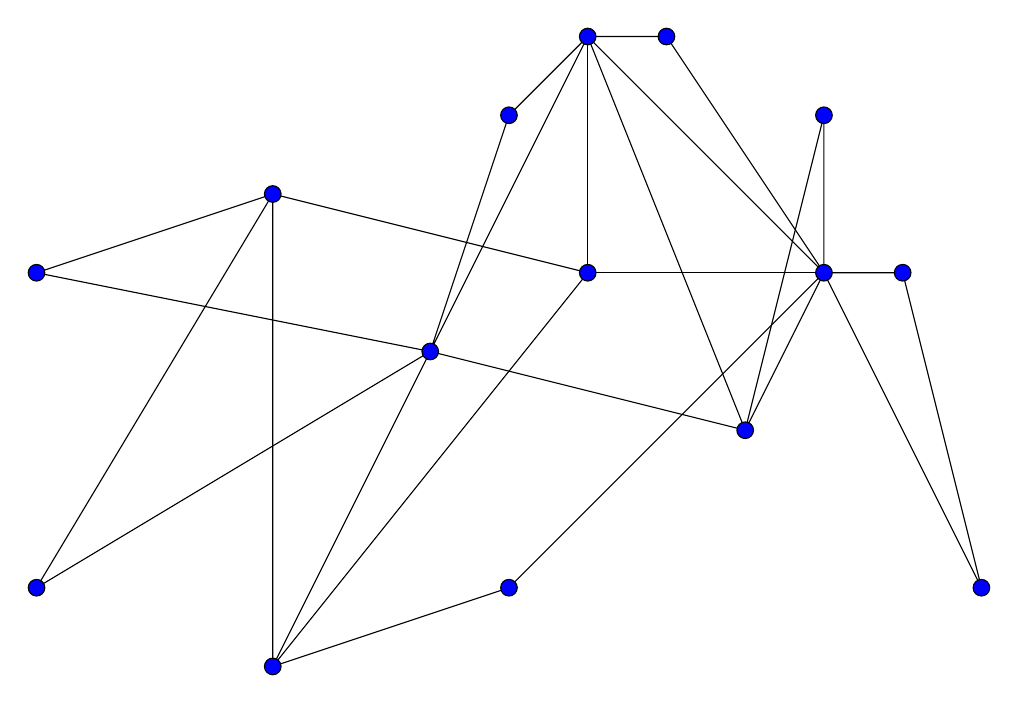
\begin{tikzpicture}
	\tikzstyle{every node}=[circle, draw, fill=blue, inner sep=0pt, minimum width=6pt]
    	  
	\draw (1, 2) -- (4, 7)
		  (1, 2) -- (6, 5);
		  
	\draw (1, 6) -- (4, 7)
		  (1, 6) -- (6, 5);

	\draw (4, 7) -- (4, 1)
		  (4, 7) -- (8, 6);

	\draw (4, 1) -- (6, 5)
		  (4, 1) --(8, 6)
		  (4, 1) -- (7, 2);
		  
	\draw (6, 5) -- (7, 8)
		  (6, 5) -- (8, 9)
		  (6, 5) -- (10, 4);
		  
	\draw (7, 2) -- (11, 6);
	
	\draw (7, 8) -- (8, 9);

	\draw (8, 6) -- (11, 6)
		  (8, 6) -- (8, 9);
		  
	\draw (8, 9) -- (9, 9)
		  (8, 9) -- (11, 6)
		  (8, 9) -- (10, 4);
		  
	\draw (9, 9) -- (11, 6);
	
	\draw (10, 4) -- (11, 6)
		  (10, 4) -- (11, 8);
		  
	\draw (11, 6) -- (11, 8)
		  (11, 6) -- (12, 6)
		  (11, 6) -- (13, 2);
		  
	\draw (12, 6) -- (13, 2);
	
    \draw (1, 2) node {} 
    	  (1, 6) node {} 
    	  (4, 7) node {} 
    	  (4, 1) node {} 
    	  (6, 5) node {} 
    	  (7, 2) node {} 
    	  (7, 8) node {} 
    	  (8, 6) node {} 
    	  (8, 9) node {} 
    	  (9, 9) node {} 
    	  (10, 4) node {} 
    	  (11, 6) node {} 
    	  (11, 8) node {} 
    	  (12, 6) node {} 
    	  (13, 2) node {};

\end{tikzpicture}\end{center}

\begin{center}\small Рис. \images. Эйлеров граф\end{center}	
	
	Эйлеровы графы имеют в качестве <<собратьев по несчастью>> гамильтоновы графы~---~графы, в которых можно обойти все вершины, 
	побывав в каждой ровно один раз. Однако несмотря на простоту первых из них, вторые не поддаются никакой классификации и до сих пор неизвестно, 
	есть ли оптимальный алгоритм, который мог бы ответить на вопрос: гамильтонов ли наш граф или нет? 
	Говоря об оптимальности, математики подразумевают достаточно формальные понятия. О них мы тоже упомянем немного ниже.
	
	Своим появлением гамильтонов цикл обязан задаче о коммивояжёре, в которой торговец должен был обойти все города, побывав в каждом ровно один раз. 
	С тех пор появилось много задач, для решения которых нужно найти гамильтонов цикл, так что можно считать, 
	что этот путь развития теории графов был вполне успешным.	
	
	Сам Гамильтон сформулировал и решил следующую задачу: можно ли обойти додекаэдр, побывав в каждой вершине единожды. 
	Одно из решений есть на рис. 13.
	
\begin{center}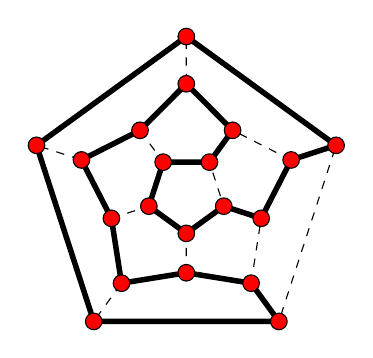
\begin{tikzpicture}
	\tikzstyle{every node}=[circle, draw, fill=red, inner sep=0pt, minimum width=6pt]	
	
	\draw [line width=0.7mm] (126:0.5) -- (198:0.5) -- (270:0.5) -- (342:0.5) -- (342:1.0) -- (18:1.4) -- (18:2.0) -- (90:2.0) -- (162:2.0) -- (234:2.0) -- (306:2.0) -- (306:1.4) -- (270:1.0) -- (234:1.4) -- (198:1.0) -- (162:1.4) -- (126:1.0) -- (90:1.4) -- (54:1.0) -- (54:0.5) -- (126:0.5);

    \draw [dashed]  \foreach \x in {54,126,...,342}
    {
    	
    	(\x:1.0) -- (\x:0.5) -- (\x+72:0.5)
    	(\x-36:1.4) -- (\x:1.0) -- (\x+36:1.4) -- (\x+36:2.0) -- (\x-36:2.0)
    };	
    \draw \foreach \x in {54,126,...,342}
    {
    	(\x:0.5) node {}
    	(\x:1.0) node {}
    };
    \draw \foreach \x in {18,90,...,306}
    {
    	(\x:1.4) node {}
    };
    \draw \foreach \x in {18,90,...,306}
    {
    	(\x:2.0) node {}
    };
\end{tikzpicture}

	\small Рис. \images. Гамильтонов цикл в додекаэдре
\end{center}
	
\begin{paracol}{2}
	\textbf{Теорема о четырёх красках} утверждает, что любую карту можно раскрасить в четыре цвета так, что любая страна будет раскрашена в один цвет, 
	а любые соседние страны будут раскрашены в разные цвета. Фрэнсис Гутри, сформулировавший эту задачу, изначально имел перед собой цель 
	только раскрасить карту Англии. Он заметил, что меньше четырёх красок не хватит для этого. 

\begin{testquestion}	
	Можете ли вы посмотреть на схематический рисунок Великобритании и объяснить, почему меньше четырёх красок не хватит?
\end{testquestion}
	
	В $1976$ году эту теорему успешно доказали Кеннет Аппел и Вольфганг Хакен, однако то решение, которое они предложили, 
	вызвало сильный резонанс среди коллег. Дело было в том, что математики свели доказательство к проверке около двух тысяч 
	графов на раскраску, но очень трудоёмко~---~проверять все эти случаи вручную, поэтому был написан машинный код, который 
	и должен был справиться с задачей. Такой подход вызвал бурю возмущений среди их коллег...
	
\switchcolumn

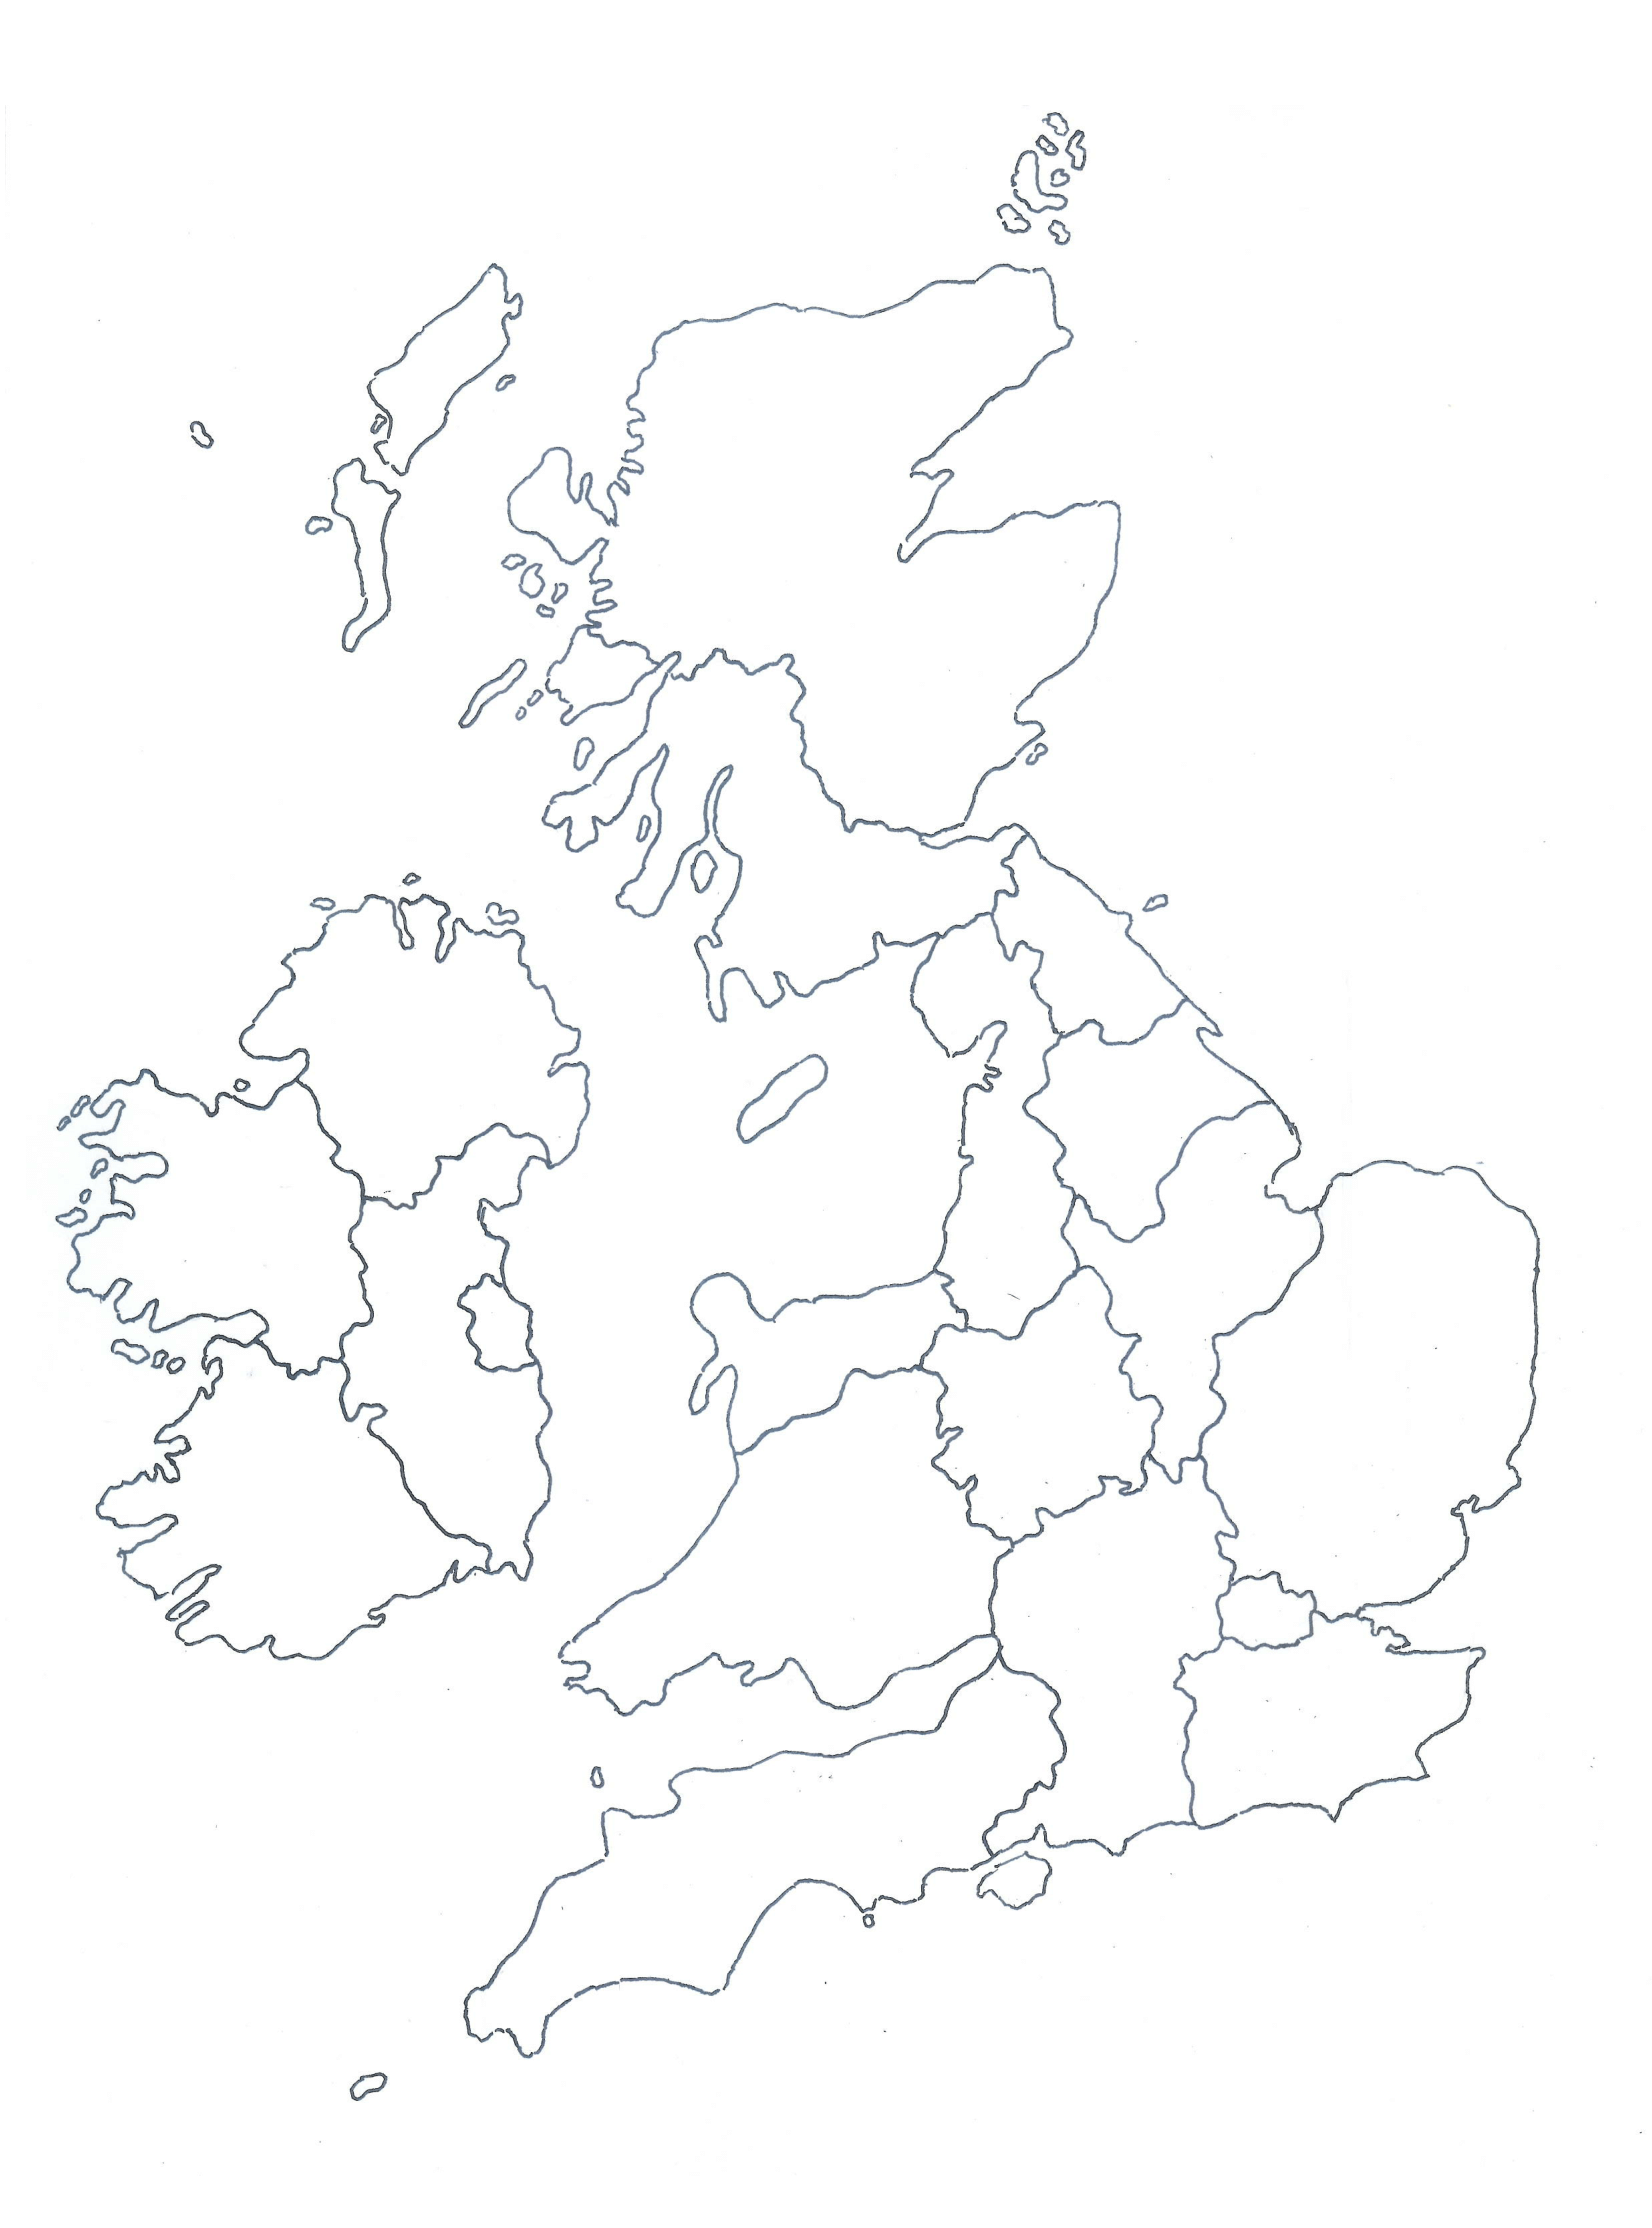
\includegraphics[width=8cm, height=24cm,keepaspectratio]{chapters/1/images/England}

\begin{center} \small Рис. \images. Схематическое изображение частей Великобритании (пропорции не сохранены) \end{center}
\end{paracol}
\refstepcounter{images}

	Фактически Аппел и Хакен поставили перед научным миром непростой вопрос: можно ли считать доказательство, 
	использующее работу компьютера, строгим, правильным, с формальной точки зрения? 
	
	Долгое время всё сообщество не могло принять такой подход даже по отношению к теореме о четырёх красках, но в $1997$ 
	году Робертсон, Сандерс, Сеймур и Томас предложили более простое доказательство теоремы, которое безвозвратно поместило эту 
	теорему в список <<доказанных>>. К настоящему моменту почти все математики согласились с обоснованным использованием 
	электронных носителей для завершения доказательства сложных теорем.
	
	\textbf{Задача о клике} была сформулирована в $1972$ году Ричардом Карпом. Причиной её появления можно считать дикое развитие 
	теории вычислительных систем, начавшееся в середине $50$-х годов \RNumb{20} века и продолжающееся до сих пор. Условие у этой задачи 
	следующее: предложите оптимальный алгоритм по нахождению максимального полного подграфа произвольного графа. Под полным подграфом 
	подразумевается граф, в котором любые две вершины соединены ровно одни ребром и нет петель, то есть рёбер выходящих и 
	входящих в одну и ту же вершину.
	
	По своей сути задача о клике говорит об оптимальном алгоритме. Ясно, что можно перебрать все возможные подграфы 
	и проверить для каждого, является ли он полным, однако это не будет оптимальным алгоритмом. Критерий оптимальности 
	в этом случае состоит в том, что время, которое мы тратим на работу алгоритма, есть функция, зависящая от длины входных 
	данных. И по этому делению задача о клике относится к $NP$-полным задачам. В этот класс входят те задачи, которые за 
	полиномиальное время не решаются, но любое их решение можно проверить на правильность за полиномиальное время.
	
\begin{center}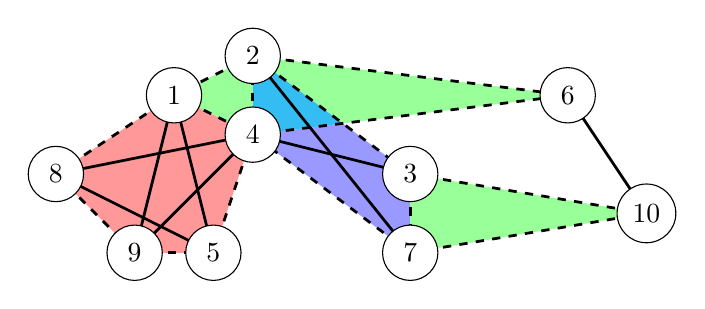
\begin{tikzpicture}
	\tikzstyle{every node}=[minimum width=20pt]	

	\fill [draw=none, fill=green!40] (2, -0.5) -- (3, -1) -- (3, 0) -- (2, -0.5);
	\fill [draw=none, fill=blue!40] (5, -2.5) -- (3, -1) -- (3, 0) -- (5, -1.5);
	\fill [draw=none, fill=green!40] (3, -1) -- (3, 0) -- (7, -0.5);
	\fill [draw=none, fill=red!40] (2, -0.5) -- (3, -1) -- (2.5, -2.5) -- (1.5, -2.5)  -- (0.5, -1.5);
	\fill [draw=none, fill=green!40] (5, -1.5) -- (5, -2.5) -- (8, -2);
	
	\begin{scope}
		\clip (5, -2.5) -- (3, -1) -- (3, 0) -- (5, -1.5);
		\clip (3, -1) -- (3, 0) -- (7, -0.5);
		\fill[color=cyan!80] (3,0) rectangle (5,-2);
	\end{scope}	
	
	\draw (2, -0.5) edge [dashed, line width=0.35mm] (3, -1) 
		  (3, -1)   edge [dashed, line width=0.35mm] (3, 0) 
		  (3, 0)    edge [dashed, line width=0.35mm] (2, -0.5);

	\draw (3, -1)   edge [dashed, line width=0.35mm] (7, -0.5) 
		  (3, 0)    edge [dashed, line width=0.35mm] (7, -0.5);
	
	\draw (3, 0)    edge [dashed, line width=0.35mm] (5, -1.5) 
		  (5, -1.5) edge [dashed, line width=0.35mm] (5, -2.5) 
		  (5, -2.5) edge [dashed, line width=0.35mm] (3, -1)
		  (3, 0)  edge [line width=0.35mm] (5, -2.5) 
		  (3, -1) edge [line width=0.35mm] (5, -1.5);

	
	\draw (2, -0.5)   edge [dashed, line width=0.35mm] (0.5, -1.5) 
		  (0.5, -1.5) edge [dashed, line width=0.35mm] (1.5, -2.5) 
		  (1.5, -2.5) edge [dashed, line width=0.35mm] (2.5, -2.5)
		  (2.5, -2.5) edge [dashed, line width=0.35mm] (3, -1)
		  (2, -0.5)   edge [line width=0.35mm] (1.5, -2.5) 
		  (2, -0.5)   edge [line width=0.35mm] (2.5, -2.5)
		  (0.5, -1.5) edge [line width=0.35mm] (3, -1) 
		  (0.5, -1.5) edge [line width=0.35mm] (2.5, -2.5)
		  (1.5, -2.5) edge [line width=0.35mm] (3, -1);
		  
	\draw (5, -1.5) edge [dashed, line width=0.35mm] (8, -2) 
		  (5, -2.5) edge [dashed, line width=0.35mm] (8, -2);

	\draw (8, -2) edge [line width=0.35mm] (7, -0.5);
		  
	\draw (2, -0.5)   node[circle, draw, fill=white] {1}
		  (3, 0)      node[circle, draw, fill=white] {2}
		  (5, -1.5)   node[circle, draw, fill=white] {3}
		  (3, -1)     node[circle, draw, fill=white] {4}
		  (8, -2)     node[circle, draw, fill=white] {10}
		  (7, -0.5)   node[circle, draw, fill=white] {6}
		  (5, -2.5)   node[circle, draw, fill=white] {7}
		  (0.5, -1.5) node[circle, draw, fill=white] {8}
		  (1.5, -2.5) node[circle, draw, fill=white] {9}
		  (2.5, -2.5) node[circle, draw, fill=white] {5};
\end{tikzpicture}

	\small Рис. \images. Произвольный граф с изображенными кликами
\end{center}

	Это далеко не все задачи, которые встречались по ходу развития теории графов. 
	К ним также можно отнести гипотезу Хадвигера, гипотезу Харари, гипотеза Конвея о трекле.
	
	Подытожим, в этом параграфе мы проследили за процессом становления теории графов и теории алгоритмов, познакомились с 
	неформальным определением графа и обсудили некоторые серьёзные теоремы, с которыми сталкивались математики по мере развития теории графов.